\documentclass[11pt]{beamer}
\usetheme{Pittsburgh}
\usepackage[utf8]{inputenc}
\usepackage[english]{babel}
\usepackage{amsmath}
\usepackage{amsfonts}
\usepackage{amssymb}
\usepackage{mathrsfs} 
\usefonttheme[onlymath]{serif}

\defbeamertemplate*{title page}{customized}[1][]
{
  \usebeamercolor[fg]{titlegraphic}\inserttitlegraphic
  \flushleft
  \medskip
  \usebeamerfont{title}\inserttitle\par
  \medskip
  \usebeamerfont{subtitle}\usebeamercolor[fg]{subtitle}\insertsubtitle\par
  \vfill
  \usebeamerfont{author}\insertauthor\par
  \usebeamerfont{institute}\insertinstitute\par
  \medskip
  \usebeamerfont{date}\insertdate\par

}
\newenvironment{proenv}{\only{\setbeamercolor{local structure}{fg=green}}}{}
\newenvironment{conenv}{\only{\setbeamercolor{local structure}{fg=red}}}{}

\setbeamertemplate{footline}[text line]{%
  \parbox{\linewidth}{\vspace*{-8pt}MSI SS14\hfill\insertshortauthor\hfill\insertframenumber}}
\setbeamertemplate{navigation symbols}{}

\titlegraphic{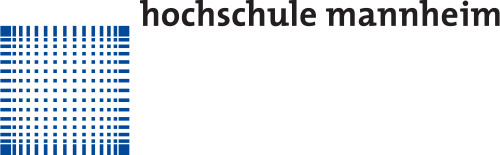
\includegraphics[scale=0.25]{logo.png}}
\author{Horst Schneider, Patrick Beedgen}
\title{Understanding Eventual Consistency}
\subtitle{MSI Presentation SS2014}
\institute{Hochschule Mannheim} 
\date{June 17th, 2014} 
\begin{document}

\begin{frame}
\titlepage
\end{frame}

\begin{frame}
\frametitle{Introduction}
\begin{quotation}
" ...the 
storage system guarantees that if no 
new updates are made to the object, 
eventually all accesses will return the 
last updated value"
\linebreak
--W. Vogels (2009)
\end{quotation}
\end{frame}



\begin{frame}
\frametitle{Introduction}
\framesubtitle{Interpretations of Eventual Consistency}
\begin{footnotesize}

\begin{block}{Interpretation 1}
\begin{quotation}
"When you read data[...], the response might not reflect the results of a recently completed write operation. The response might include some stale data. Consistency across all copies of the data is usually reached within a second; so if you repeat your read request after a short time, the response returns the latest data."
\end{quotation}
\end{block}

\begin{block}{Interpretation 2}
\begin{quotation}
"This sort of system we term “single writer eventual consistency”.  So what are its properties? \linebreak (1) A client could read stale data.\linebreak (2) The client could see out-of-order write operations. [...] So this is our weakest form of consistency - eventually consistent with out of order reads in the short term."
\end{quotation}
\end{block}
\end{footnotesize}
\end{frame}


\begin{frame}
\frametitle{Introduction}
\framesubtitle{Interpretations of Eventual Consistency}
\begin{footnotesize}
\begin{block}{DynamoDB Documentation}
\begin{quotation}
"When you read data[...], the response might not reflect the results of a recently completed write operation. The response might include \textbf{some stale data}. Consistency across all copies of the data is \textbf{usually reached within a second}; so if you repeat your read request after a short time, the response returns the latest data."
\end{quotation}
\end{block}

\begin{block}{MongoDB Documentation}
\begin{quotation}
"This sort of system we term “single writer eventual consistency”. So what are its properties?\linebreak (1)\textbf{A client could read stale data}. \linebreak(2)The client could see out-of-order write operations.[...]\linebreak So this is our weakest form of consistency - eventually consistent with \textbf{out of order reads} in the short term."
\end{quotation}
\end{block}
\end{footnotesize}
\end{frame}

\begin{frame}
\frametitle{Problems}
\begin{itemize}
\item disparate and low-level formalisms\linebreak 
\textit{consistency model is tied to system implementation}
\pause
\item weak guarantees\linebreak 
\textit{in realistic scenarios updates \textbf{never} stop}
\pause
\item conflict resolution policies\linebreak 
\textit{resolution of conflicts in multiple replicas}
\pause
\item combinations of different consistency levels\linebreak 
\textit{strong consistency may be needed at certain times} 
\end{itemize}
\pause
\begin{large}
\ensuremath{\Rightarrow}
\end{large}
some sort of formalism is needed to define semantics of Eventual Consistency
\end{frame}

\begin{frame}
\frametitle{Agenda}
\tableofcontents
\end{frame}

\section{Replicated Data Types}

\begin{frame}
\frametitle{Replicated Data Types}
\begin{itemize}
\item a replicated database stores \textbf{objects} \(\mathrm{Obj} = \{x,y,\dots\} \)
\pause
\item every object \(x \in \mathrm{Obj}\) has
\begin{itemize}
\item a \textbf{value} \(\in \mathrm{Val}\)
\item a \textbf{type} type\((x) \leftrightarrow \tau \)
\item \textbf{operations} \(\mathrm{Op}_{\mathrm{type}(x)}\) that a client can perform on it
\pause
\end{itemize}
\item two examples: Int Register \textbf{intreg}, Counter \textbf{ctr}
\end{itemize}

\begin{align*}
\mathrm{Op}_\mathrm{ctr} &= \mathrm{\{rd, inc\}} \\
\mathrm{Op}_\mathrm{intreg} &= \mathrm{\{rd, wr(}k \mathrm{)|} k \in \mathbb{Z} \mathrm{\}}
\end{align*}
\end{frame}

\begin{frame}
\frametitle{Replicated Data Types}
\framesubtitle{Sequential Data Type Specification}
in a \textit{strongly consistent system}, the semantics of a data type can be specified by a function: \\
\begin{equation*}
S_{\tau}: \mathrm{Op}_\tau^+ \rightarrow \mathrm{Val}
\end{equation*}
\pause
example:
\begin{align*}
S_{\mathrm{intreg}} \mathrm{(\sigma\ wr(}k\mathrm{))} &= S_{\mathrm{ctr}} \mathrm{(\sigma\ inc)} = \bot; \\
\onslide<3->{S_{\mathrm{ctr}} \mathrm{(\sigma rd)} &= \mathrm{(number\ of\ inc\ operations\ in\ \sigma);} \\}
\onslide<4->{
S_{\mathrm{intreg}} \mathrm{(\sigma rd)} &= k;\ \mathrm{if\ wr(0) \sigma = \sigma_1 wr(}k\mathrm{) \sigma_2\ and} \\
 & \mathrm{\sigma_2 \ does\ not\ contain\ wr\ operations}
 }
\end{align*}
(e.g. \(\sigma =\{ \mathrm{rd\ rd\ wr(5)\ wr(6)\ rd\} }\) or \(\sigma =\{ \mathrm{rd\ rd\ inc\ inc\ rd\} } \) )

\end{frame}

\begin{frame}
\frametitle{Replicated Data Types}
\framesubtitle{Semantics of Eventual Consistency}
\begin{itemize}
\item semantics of eventually consistent systems are harder to formalize
\item concurrent operations on the same object happen on multiple replicas
\item each replica executes operations immediately, updating other replicas later \(\rightarrow\) \textbf{conflicts}
\item different conflict resolution strategies for replicated data types
\end{itemize}
\end{frame}

\begin{frame}
\frametitle{Replicated Data Types}
\framesubtitle{Conflict Resolution Strategies}
\begin{columns}
\begin{column}{5cm}
\begin{figure}
\includegraphics<1-2>[scale=0.25]{update_replicas_highres_1_no_strategy.png}
\includegraphics<3>[scale=0.25]{update_replicas_highres_2_order.png}
\includegraphics<4->[scale=0.25]{update_replicas_highres_3_flag.png}
\end{figure}
\end{column}
\begin{column}{5cm}
\pause
\begin{enumerate}
\item make concurrent operations commutative
\pause
\item order concurrent operations
\pause
\item flag conflicts (let the user decide)
\pause
\item resolve conflicts semantically
\end{enumerate}
\end{column}
\end{columns}
\end{frame}

\begin{frame}
\frametitle{Replicated Data Types}
\framesubtitle{Replicated Data Type Specification}
\begin{itemize}
\item \(S_{\tau}\) is not strong enough to formalize these strategies
\item \textbf{visibility} and \textbf{order} of preceding operations have to be included
\pause
\item \(F_\tau\): takes an \textbf{operation context} \(C\) and returns a value
\end{itemize}

\begin{center}
\(F_\tau(C) \in \mathrm{Val}\) \\
\end{center}
\pause
\begin{itemize}
\item \(C\) provides preceding operations with \textbf{visibility} and \textbf{arbitration relations}:
\end{itemize}

\begin{center}
\(C = (f, V, \mathrm{ar}, \mathrm{vis})\) \\
\pause
\(u \xrightarrow{\mathrm{vis}} v, \mathrm{vis} \subseteq V \times V  \) \\
\(u \xrightarrow{\mathrm{ar}} v, \mathrm{ar} \subseteq V \times V  \)
\end{center}

\end{frame}

\begin{frame}
\frametitle{Replicated Data Types}
\framesubtitle{Replicated Data Type Specification}
example: Strategy \textbf{Make Concurrent Calls Commutative}
\begin{align*}
F_{\mathrm{ctr}} \mathrm{(inc}, V, \mathrm{vis, ar)} &= \bot; \\
F_{\mathrm{ctr}} \mathrm{(rd}, V, \mathrm{vis, ar)} &= \mathrm{(the\ number\ of\ inc\ operations\ in\ } V);
\end{align*}
\pause
example: Strategy \textbf{Order Concurrent Operations}
\begin{align*}
F_{\mathrm{intreg}} (f, V, \mathrm{vis, ar)} &= S_{\mathrm{intreg}}(V^{\mathrm{ar}} f) \\
&(S_{\tau}\ :\ \mathrm{Op}_\tau^+ \rightarrow \mathrm{Val})
\end{align*}
\end{frame}

\begin{frame}
\frametitle{Replicated Data Types}
\framesubtitle{Replicated Data Type Specification}
example: Strategy \textbf{Flag Conflicts}
\begin{center}

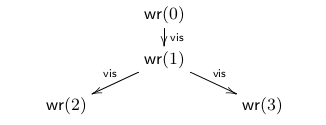
\includegraphics[scale=0.6]{mvr.png}
\\
writes on a multi value register

\end{center}
\end{frame}

\section{Axiomatic Specification Framework}

\begin{frame}
\frametitle{Axiomatic Specification Framework}
\framesubtitle{Session and Action}
\begin{itemize}
\item a single client may do several changes to the same object
\item \textbf{sessions} provide a way to track client identity for operations
\item an \textbf{action} is a tuple \((e,s,[x.f:k])\)
\begin{itemize}
\item \(e\): unique identifier
\item \(s\): session id \(\in \mathrm{SId}\)
\item \([x.f:k]\): object, operation and return value
\end{itemize}
\end{itemize}
\pause
example:

\begin{center}
\(a = (1af3c, 17, [x.rd: k]);\ \mathrm{type(}x\mathrm{)} = \mathrm{intreg}\)
\end{center}
\end{frame}

\begin{frame}
\frametitle{Axiomatic Specification Framework}
\framesubtitle{History and Execution}
\begin{itemize}
\item the set of all actions that happen in a database is denoted as \(\mathrm{Act}\)
\item a \textbf{history} \((A,\mathrm{so})\) is a set of actions \(A \subseteq \mathrm{Act}\) and a \textbf{session order} relation \(\mathrm{so} \subseteq A \times A \)
\item an \textbf{execution} \(X = (A, \mathrm{so, vis, ar})\) enhances the history with visibility and arbitration relations
\item we can now extract an operation context for any action in any session, providing a deterministic return value
\end{itemize}

\end{frame}

\begin{frame}
\frametitle{Axiomatic Specification Framework}
\framesubtitle{Levels of Eventual Consistency}
\begin{itemize}
\item with replicated data types we can define multiple forms of Eventual Consistency
\begin{itemize}
\item Basic Eventual Consistency
\item Session Guarantees
\item Causality
\end{itemize}
\item every form contains multiple axioms
\item more axioms mean stronger consistency
\end{itemize}
\end{frame}

\begin{frame}
\frametitle{Axiomatic Specification Framework}
\framesubtitle{Basic Eventual Consistency Axioms}
\begin{itemize}
\item axioms a database implementation has to enforce to offer \textbf{basic eventual consistency} 
\item Well Formedness Axioms
\begin{itemize}
\item SOwf: \textbf{so} \textit{is the union of transitive, irreflexive and total orders
on actions by each session}
\item VISwf: \(\forall a,b. \text{ } a \xrightarrow[]{\text{ vis }}b \Rightarrow obj(a) = obj(b) \)
\item ARwf: \(\forall a,b. \text{ } a \xrightarrow[]{\text{ ar }} b \Rightarrow obj(a) = obj(b) \)
\end{itemize}
\end{itemize}
\end{frame}

\begin{frame}
\frametitle{Axiomatic Specification Framework}
\framesubtitle{Basic Eventual Consistency Axioms}
\begin{itemize}
%\item Data Type Axiom(RVAL): \linebreak \(\forall a \in A. \text{ } \mathrm{rval}(a) = F \mathrm{_{type(a)}} (\mathrm{ctxt}(a))\)
\item Basic Eventual Consistency axioms:
\begin{itemize}
\item THINAIR: \(\mathrm{so} \cup \mathrm{vis} \text{ } \mathrm{is} \text{ } \mathrm{anticyclic} \) 
\pause
\begin{center}
\textbf{not} possible in THINAIR:\\
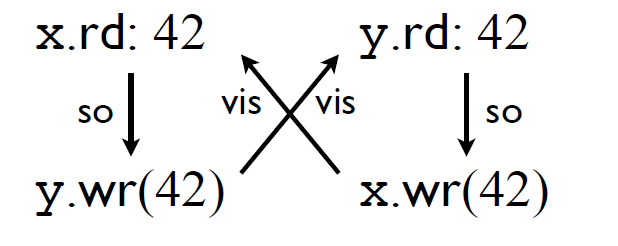
\includegraphics[scale=0.25]{thinair.png}
\end{center}
\pause
\item EVENTUAL: \linebreak \(\forall a \in A. \text{ } \neg(\exists \mathrm{infinitely} \text{ } \mathrm{many} \text{ } b  \in A. \text{ } \mathrm{same}(a,b)) \wedge \neg(a \xrightarrow[]{\text{vis}} b)) \)
\end{itemize}
\end{itemize}
\end{frame}

\begin{frame}
\frametitle{Axiomatic Specification Framework}
\framesubtitle{Problem with basic eventual consistency}
TODO: Image explaining photo/noboss example from paper
\end{frame}

\begin{frame}
\frametitle{Axiomatic Specification Framework}
\framesubtitle{Session guarantees}
\begin{itemize}
\item with basic eventual consistency we still might be reading values out of order
\item axioms that formalise that all operation within a session keep the current context consistent:
\begin{itemize}
\item Read Your Writes: \textit{An operation sees all previous operations
by the same session}
\item Writes Follow Reads in Visibility: \textit{Arbitration orders an
operation after other operations previously seen by the same session}
\item ... etc.
\end{itemize}
\end{itemize}
\end{frame}

\begin{frame}
\frametitle{Axiomatic Specification Framework}
\framesubtitle{Causality Axioms}
\begin{itemize}
\item Per-object-causal-visibility:
\textit{POCV guarantees that an operation sees all operations
on the same object that causally affect it}
\pause
\begin{center}
\begin{figure}
\textbf{not} allowed in POCV:
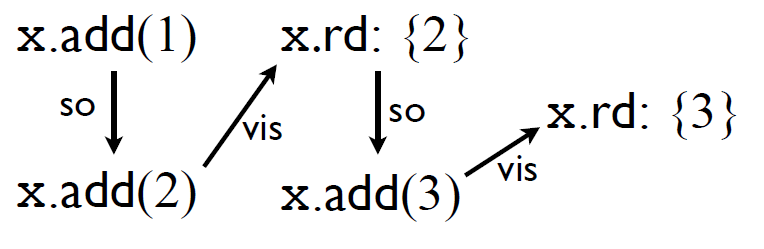
\includegraphics[scale=0.4]{pocv.png}
\end{figure}
\end{center}
\pause
\item Per-object-causal-arbitration:
\textit{POCA correspondingly
restricts the arbitration relation}
\end{itemize}
\end{frame}

\section{Consistency Strengthening Interfaces}

\begin{frame}
\frametitle{Consistency Strengthening Interfaces}
\framesubtitle{Online Shopping}
\begin{itemize}
\item almost everybody does online shopping
\begin{itemize}
\item we put items in our shopping cart
\item we pay them
\item we continue shopping.. or not
\end{itemize}
\end{itemize}
\pause
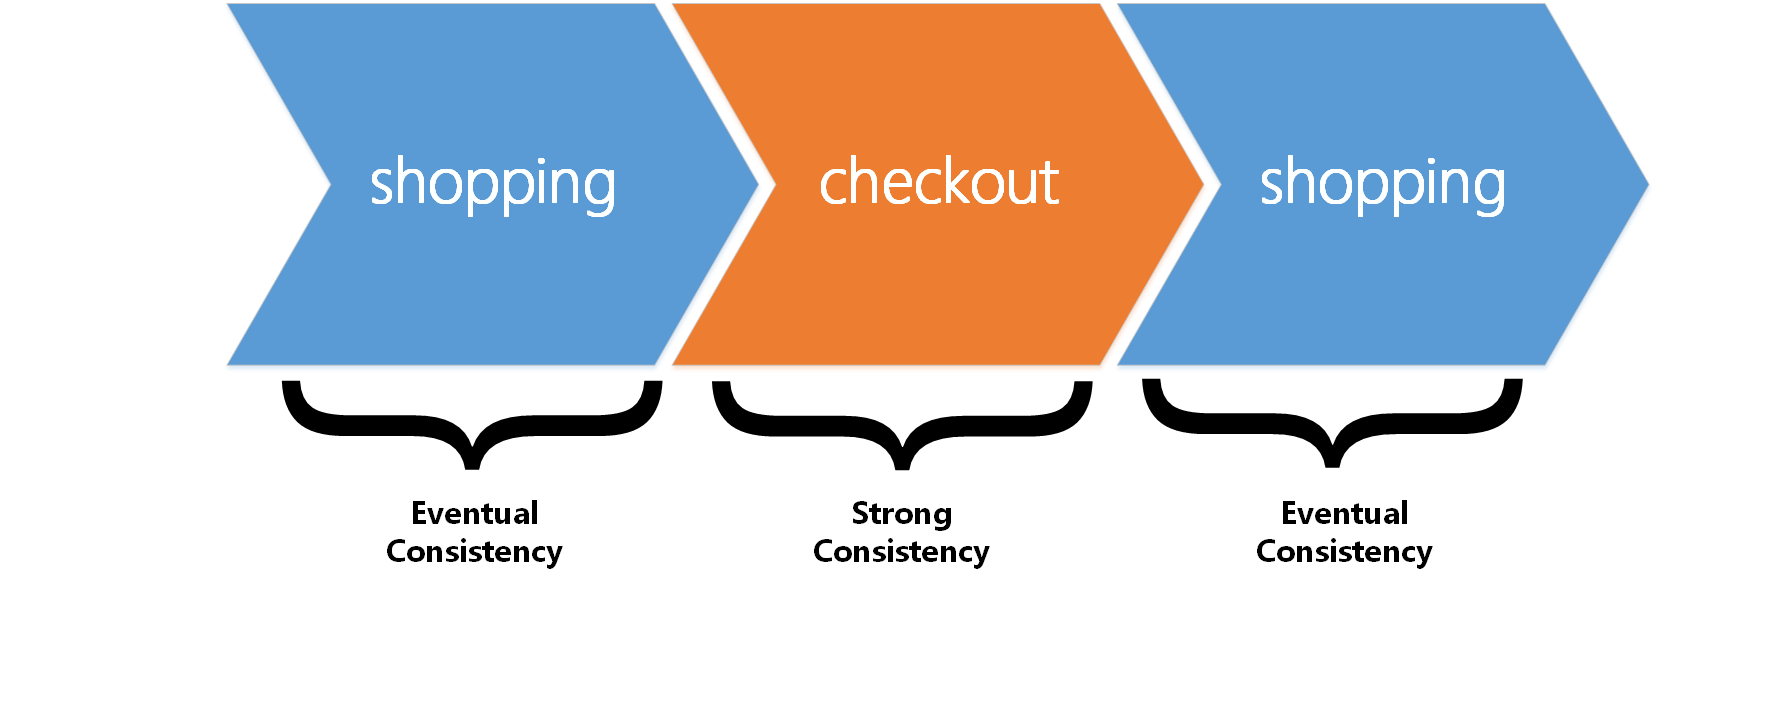
\includegraphics[scale=0.25]{shopping_example.png} \linebreak
\pause
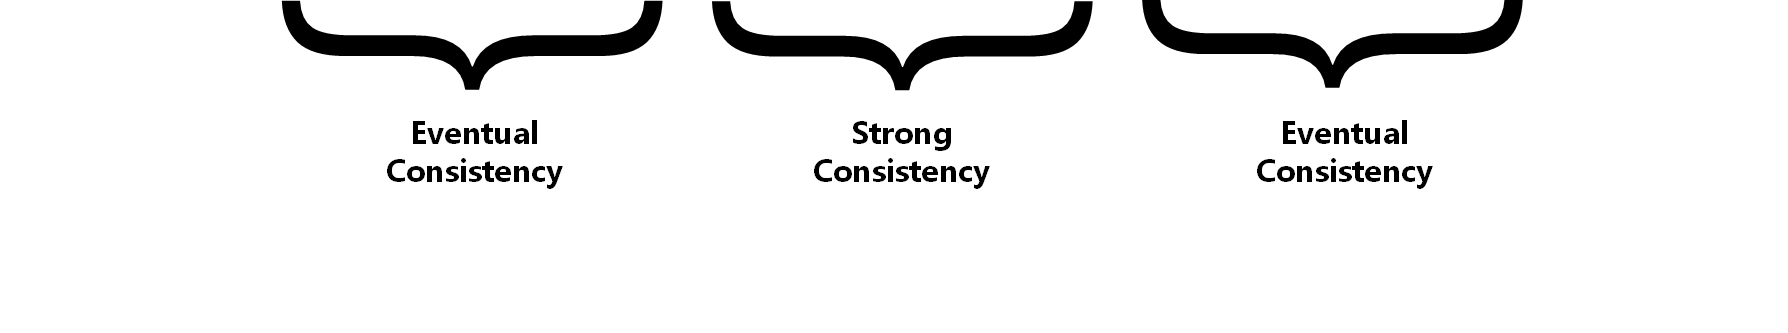
\includegraphics[scale=0.25]{shopping_example_lower.png}
\end{frame}

\begin{frame}
\frametitle{Consistency Strengthening Interfaces}
\framesubtitle{Consistency Annotations}
\begin{itemize}
\item every \textbf{action} accepted by the database has to marked with a \textbf{consistency annotation}
\begin{center} \((e,s,[x.f\mathrm{_{\mu}}:k]) \mu \in \{ORD, CSL\}\)\end{center} 
\item either \textbf{ordinary} or \textbf{causal}
\item ordinary actions behave like we defined previously
\item causal actions make all operations performed before the annotations visible to all previous actions
\end{itemize}
\end{frame}

\begin{frame}
\frametitle{Consistency Strengthening Interfaces}
\framesubtitle{Fences}
\begin{itemize}
\item instead of annotating every single action, a \textbf{fence} can be used
\item a \textbf{fence} is an \textbf{action} where the executing replica forces all its updates on every other replica in the cluster
\begin{center} action a =  \((e,s, \mathrm{fence})\)\end{center} 
\item the execution of other actions is halted until all replicas acknowledge the receipt
\pause
\item the database behaves like a \textbf{CP} database !
\end{itemize}
\end{frame}


\section{Conclusion / Discussion}

\begin{frame}
\frametitle{Conclusion}
\begin{itemize}
\item<pro@1-> the paper provides a formal way to \textbf{precisely specify eventually consistent systems}
\item<pro@1-> \textbf{Every aspect of a system is covered}, from data types to client interaction
\item<pro@1-> specifications are \textbf{independent of implementation details}
\item<con@1-> still \textbf{very theoretical}, no tools available to map between specifications and implementation 
\item<con@1-> the framework is \textbf{not suitable for programmers}, as it is very abstract and not easily understandable and applicable
\item<con@1-> the paper is still "work in progress"
\end{itemize}
\end{frame}

\begin{frame}
\begin{center}
\begin{Huge}
Discussion
\end{Huge}
\end{center}
\end{frame}

\end{document}
